\section{Current contributions}

\subsection{Proof of Concept}

\begin{figure}[!b]
   \begin{center}
      \includegraphics[width=0.3\columnwidth]{fig/corridor_0}
    \hfill
      \includegraphics[width=0.3\columnwidth]{fig/corridor_1}\\\vspace{5mm}
      \includegraphics[width=0.3\columnwidth]{fig/corridor_2}
    \hfill
      \includegraphics[width=0.3\columnwidth]{fig/corridor_3}
      \caption{Screen grab from the video available at~\url{https://youtu.be/4SW4j7DDxYE}.\label{fig:video}}
   \end{center}
\end{figure}




\begin{itemize}
    \item T.~Vintr, S.~Molina, J.~Fentanes, G.~Cielniak, T.~Duckett, and T.~Krajn{\'i}k, ``Spatio-temporal models for motion planning in human-populated environments,'' in \emph{Student Conference on Planning in Artificial Intelligence and Robotics}, 2017.
\end{itemize}

In \cite{vintr2017spatiotemporal} we proposed a concept of modelling human activities over the time in their natural environment.
We hypothesised that there are some patterns of human behaviour over the timeline.
As these patterns are derived from the routines and habits of humans, these patterns show periodical and continuous nature.
We also hypothesised that there are no or negligible trends in these patterns due to the nature of human habits. 
Let us consider these examples to explain periodicity and continuity of human behaviour:

... copy from mesas ...
\begin{itemize}
    \item the human  behaviour is very similar during every morning as opposed to the difference in behaviour during morning and afternoon of one randomly chosen day,
    \item human behaviour five minutes before midnight and five minutes after midnight could be probably very similar, although we compare behaviour in two different days,
    \item contrary to that, human behaviour during Sunday afternoon is probably different from behaviour on Monday afternoon.
\end{itemize}
... end ...

Such a periodical behaviour is not only forced by natural physical demands like fatigue or hunger, but also by social demands like regular working hours or the compulsory education system. 

To create the model of the time-dependent patterns of human behaviour, we need to estimate the parameters of their distribution.
As the timeline is continuous and it is not possible to repeat the experiment at the same time, the timeline is not suitable as a domain for time-dependent feature parameters estimation, especially for rare events.
The conventional approach to this task, known as time series forecasting, is to divide time-dependent events into three different components - a trend, seasonal and cyclic patterns - and analyse them separately \cite{gould2008forecasting}.
The cyclic patterns are not predictable changes in the time series, seasonal patterns are the periodical changes, and the trend is continuous growth or decrease of measured values.
To model human behaviour with the assumption of high periodicity and no trend, but with the accent to the continuity, we not only find and model dominant periodicities but also project timeline into the new multidimensional vector space.
In particular, we project every chosen periodicity into the $2d$ circle in the way, that every pattern that occurs periodically and matching chosen periodicity projects in the same position in this circle.
By this projection we solve two issues:
\begin{itemize}
    \item the time domain is constrained, and therefore it is possible to estimate distribution parameters of the time-dependent periodical patterns,
    \item and the continuity is guaranteed.
\end{itemize}

\subsubsection{Time Projection in Detail}

To prove this concept we used data of human positions during two days collected at the corridors of the School of Computer Science at the University of Lincoln.

... copy from pair ...
Data collection was performed by a mobile robot equipped with a Velodyne 3d laser range-finder.
The robot was placed at a T-shaped junction so that its laser range-finder was able to scan the three connecting corridors simultaneously.
To detect and localise people in the 3d point clouds provided by the scanner, we used an efficient and reliable person detection method~\cite{yan2017online}.
Each day contains approximately $28000$ entries, which correspond to hundreds of people walking or standing in the monitored corridors.
... end ...

The dataset consists of vectors $\left(x, y, t\right)$.
For the sake of simplicity we chose only one periodicity $T = 86400 s$ (one day), and project these vectors into the extended vector space in this way: $\left(x, y, t\right) \rightarrow \left(x, y, \cos\frac{2\pi t}{T}, \sin\frac{2\pi t}{T}\right)$.
Then we modelled the distribution by the Gustafson--Kessel Algorithm~\cite{gustafson1979fuzzy} with the number of clusters $k=30$.

\subsubsection{Conclusion}

We visualised this model of "distribution" of people at corridors in the form of a video that can be found online at [nefunkcni odkaz].
Every video frame, Figure~\ref{fig:video}, consists of $5$ minutes time frame reconstruction and the whole video consists of two days.
We can see that the model changes over time and respects corridor boundaries. 
We proved that this concept is functional.




\subsection{Warped Hypertime}

\begin{itemize}
    \item Spatiotemporal models of human activity for robotic patrolling
\end{itemize}

\begin{figure}[!b]
\begin{center}
    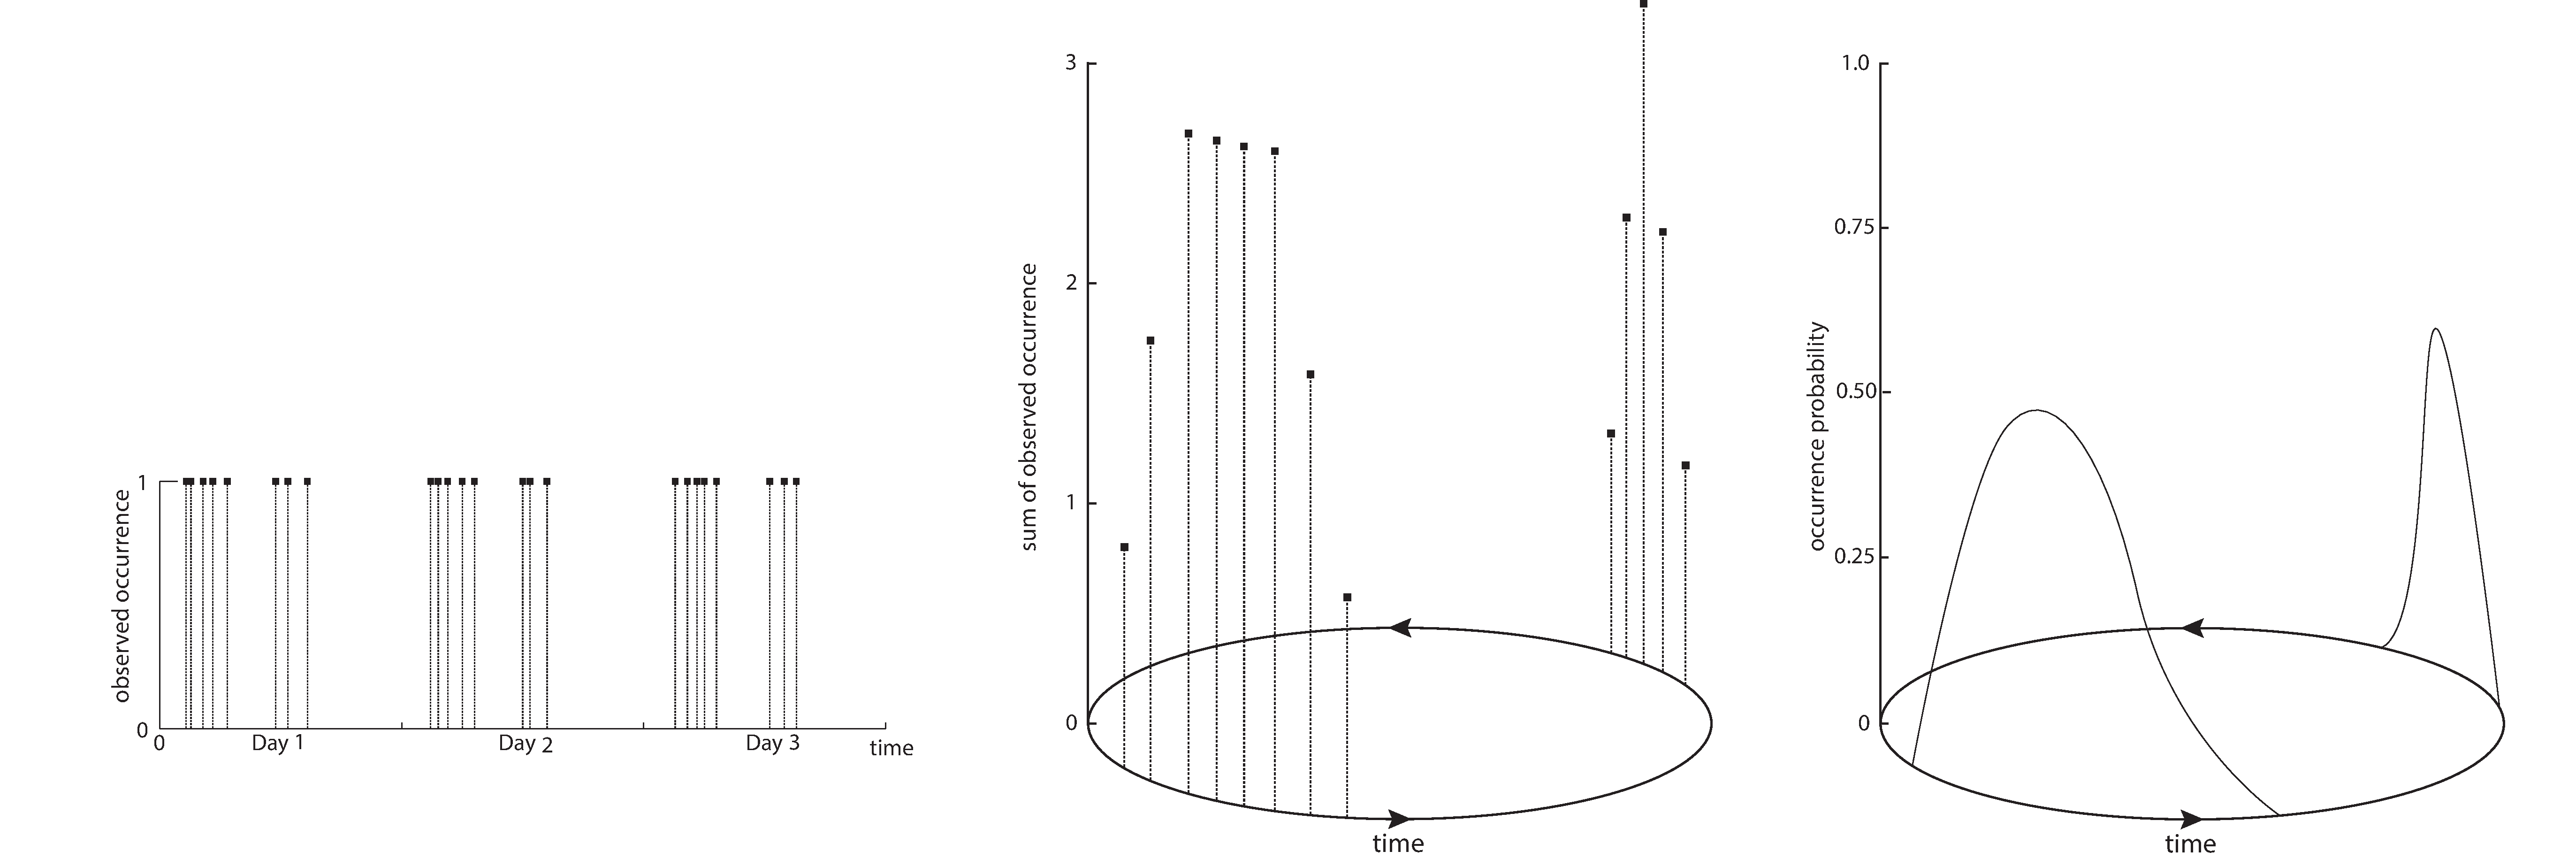
\includegraphics[width=1.0\columnwidth]{fig/hypertime_graph}
    \caption{Example of the warped hypertime projection. Positive detections during three days are projected into a warped hypertime with a one day period. The parameters of the distribution of a random time-dependent phenomenon that exhibit a periodic behaviour can be easily estimated.\label{fig:hypertime}}

\end{center}
\end{figure}



The aim of the method presented in [mesas] was to create a model of human behaviour and detect anomalous events. 
We already showed that it is possible to extend vector space of measured events by one circle, see Fig.~\ref{fig:hypertime}.
In this article, we hypothesised that it is possible to extend vector space with multiple circles and model the distribution of patterns matching different periodicities over such vector space.
To prove the concept of multiple circles extension we chose to: 
\begin{itemize}
	\item analyse the time series of human detections consisting of values one (human present) and zeros (human not present) over $18$ weeks, 
	\item and compare our approach to the FreMEn, the Frequency Map Enhancement method \cite{krajnik2017fremen} specially developed to model binomial time series, and Prophet \cite{taylor2018forecasting}, the open source, time series analysis tool created by Facebook.
\end{itemize}
We call the projection of time into the multiple circles Warped Hypertime, WHyTe.

\subsubsection{Creation of Warped Hypertime in Detail}

... copy from mesas ...
Let us have time series $R\left(t_{i}\right)$, $i = 1 \ldots n$, where $R\left(t_{i}\right) = 1$ when the sensor detects an occurrence of the studied phenomenon and $R\left(t_{i}\right) = 0$ otherwise.
Then we use the spectral analysis to find periodicities in the data. Specifically, we will use the method derived from the Frequency Map Enhancement \cite{krajnik2017fremen}.
This method is suitable to analyse time series with binary data, and it is robust to missing values.
For every considered period $T_{\tau}$, $\tau = 1 \ldots \Upsilon$, corresponding to the frequency ${f}_{\tau} = 1 / T_{\tau}$ we calculate a component of the frequency spectrum

\begin{equation}\label{eq:components}
\gamma_{\tau} = \frac{1}{n} \sum_{i = 1}^{n} (R\left(t_{i}\right)-\mu)e^{(-1j)t_{i}{f}_{\tau}2\pi},
\end{equation}

\noindent where $\mu = \frac{1}{n} \sum_{i = 1}^{n} R\left(t_{i}\right)$, sort them in descending order and return corresponding periods ordered accordingly.
... end ...

For every chosen period $T_{\tau}$ and for each $t_i$ of the original measured data we can create $2d$ warped hypertime (Fig.~\ref{fig:hypertime}) as follows:

\begin{equation}
t_i \rightarrow \left(\cos{\frac{2\pi t_{i}}{T_{\tau}}}, \sin{\frac{2\pi t_{i}}{T_{\tau}}}\right),
\end{equation}
%
where warped hypertime $\left(\cos{\frac{2\pi t_{i}}{T_{\tau}}}, \sin{\frac{2\pi t_{i}}{T_{\tau}}}\right)$ forms a circle in $2d$ plane which represent the periodicity and continuity of the occurences.
The time values of occurrences and non-occurrences with the similar position relative to periodicity $T_{\tau}$ are projected on the similar position on the circle.

During the iterative process, we extend the extended vector space with other couples of dimensions.
Such projection of $t_i$ will be denoted ${}^{@}\mathbf{t}_{i},$ where:
%
\begin{equation}\label{eqn:extension}
    {}^{@+1}\mathbf{t}_{i} = \left({}^{@}\mathbf{t}_{i}, \,\cos{\frac{2\pi t_{i}}{T_{\tau_{@+1}}}}, \, \sin{\frac{2\pi t_{i}}{T_{\tau_{@+1}}}}\right),
\end{equation}
%
in particular ${}^{2}\mathbf{t}_{i} =\left({}^{1}\mathbf{t}_{i}, \,\cos{\frac{2\pi t_{i}}{T_{\tau_2}}}, \, \sin{\frac{2\pi t_{i}}{T_{\tau_2}}}\right) =  \left(\cos{\frac{2\pi t_{i}}{T_{\tau_1}}}, \, \sin{\frac{2\pi t_{i}}{T_{\tau_1}}}, \,\cos{\frac{2\pi t_{i}}{T_{\tau_2}}}, \, \sin{\frac{2\pi t_{i}}{T_{\tau_2}}}\right),$ and
${}^{1}\mathbf{t}_{i} = \left(\cos{\frac{2\pi t_{i}}{T_{\tau_1}}}, \, \sin{\frac{2\pi t_{i}}{T_{\tau_1}}}\right)$.



\subsubsection{Conclusion}
\begin{figure}[htb]
\begin{center}
    \includegraphics[width=1.0\columnwidth]{fig/mathew_graph_90}
    \caption{Evolution of Matthews correlation coefficient using significance level $\alpha=0.1$. On the x axis there are numbers of days used to train model, on the y axes are values of Matthews correlation coefficient $\left<-1;1\right>$. A coefficient of value $1$ means correct labelling of outliers by the corresponding method.   \label{graph:mathew90}}

\end{center}
\end{figure}

In [mesas] we compare the ability of model based on warped hypertime to other approaches, especially FreMEn \cite{krajnik2017fremen} and Prophet \cite{taylor2018forecasting}. 
It was successfully compared in multiple ways (Figure~\ref{graph:mathew90}): a number of days needed to learn the cor model, the correctness of anomaly detection deduced from Matthews correlation coefficient \cite{matthews1975comparison} and robustness to the choice of significance level.
We proved that it is possible to model patterns matching different periodicities by the projection of the timeline into the multidimensional warped hypertime.
It also proved our hypothesis, that it is possible to neglect trend in time series when modelling human behaviour.


